\section{Mathematical Concept}
\frame{\sectionpage}
\begin{frame}
    \frametitle{Mathematical Concept}
    \onslide<1->{
        Let $D = \{(x_{1},y_{1}), (x_{2}, y_{2}), ... , (x_{N}, y_{N})\}$ and \\
        $T_{D,\theta}$ is a fully grown tree trained on set $D$ with using parameters $\theta$.\\
        Random Forest estimate of an observation $x^*$ is
    }
    \onslide<2->{
        \begin{block}{Majority Voting}
                \begin{center}
                    $\boldsymbol{RF}_{D, \theta_{1}, \theta_{2}, ..., \theta_{B}} (x^*) =
                    \underset{c \in Y}{argmax} \sum_{b = 1}^{B}{1(\hat{T}_{b}(x^*) = c)}$
                \end{center}
            \end{block}
    }
    \onslide<3->{
        \begin{block}{Soft Voting}
                \begin{center}
                    $\boldsymbol{RF}_{D, \theta_{1}, \theta_{2}, ..., \theta_{B}} (x^*) =
                    \underset{c \in Y}{argmax} \dfrac{1}{B}\sum_{b = 1}^{B}{\hat{p}_{D, \theta_{b}} (Y = c | X = x^*)}$
                \end{center}
                where $\hat{p}_{D, \theta_{b}} (Y = c | X = x^*)$ is the probability estimates of a tree.
            \end{block}
        
    }
\end{frame}
\begin{frame}
    \frametitle{Mathematical Concept}
    \framesubtitle{Majority Voting Illustration}
    \begin{figure}
        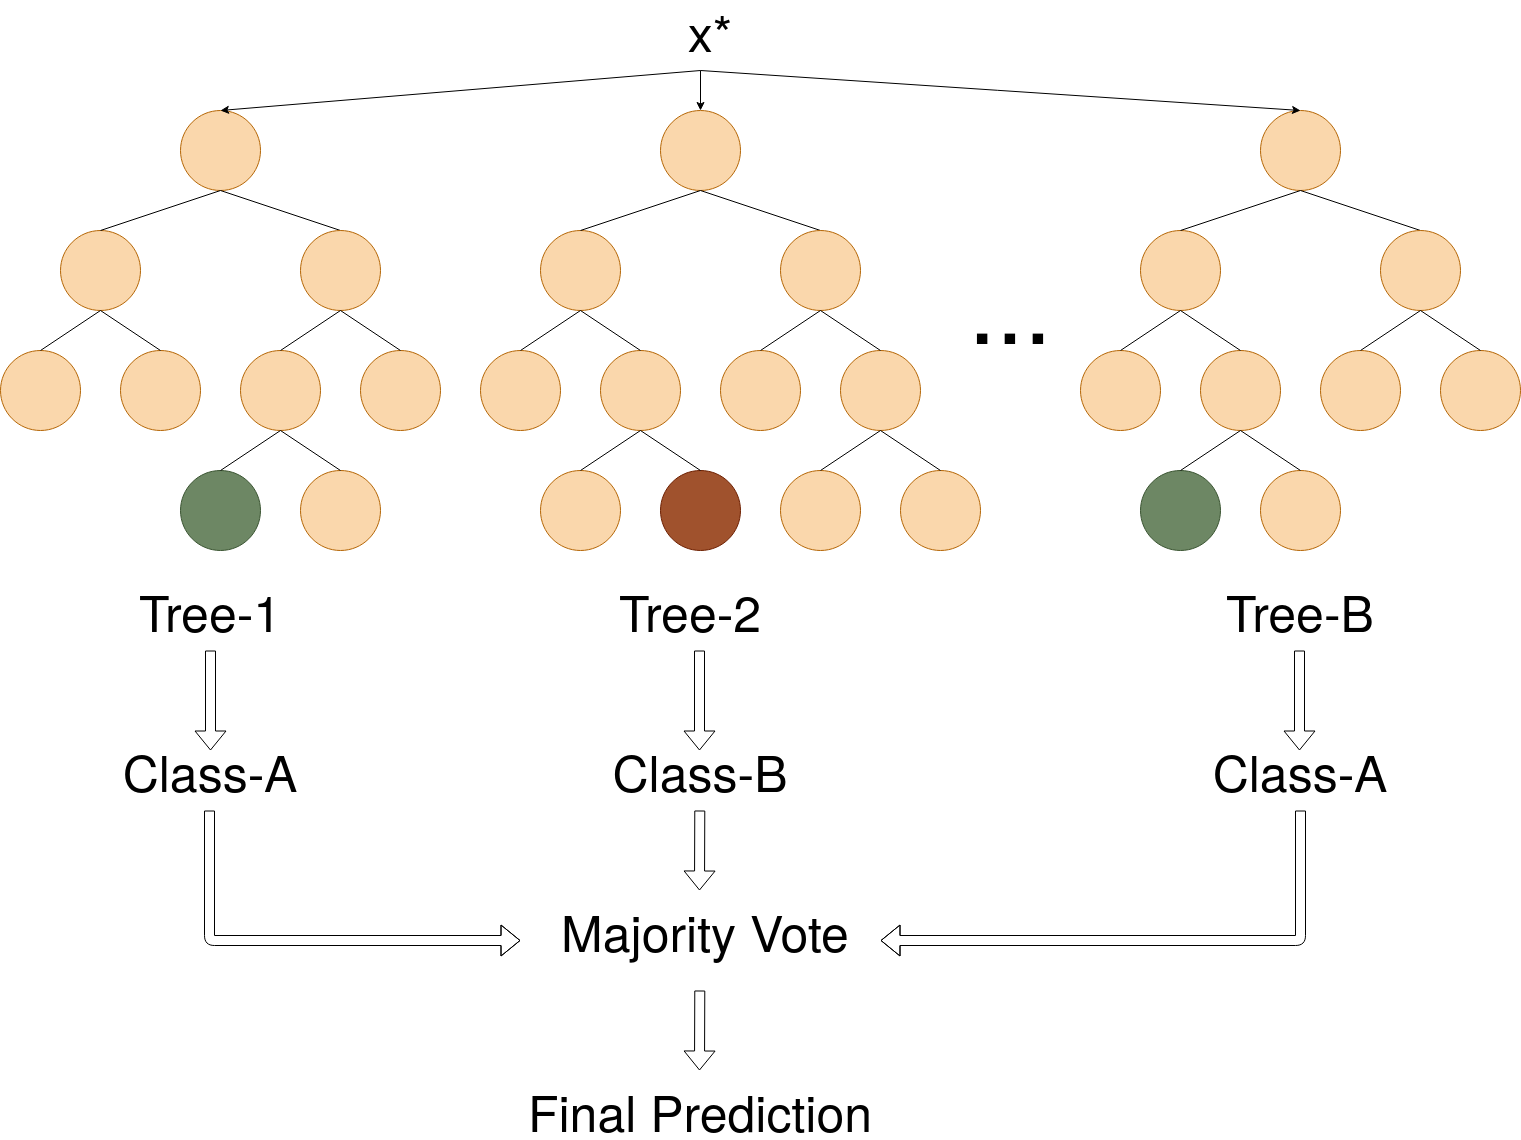
\includegraphics[height=0.7\textheight]{images/majority.png}
    \end{figure}
\end{frame}
\begin{frame}
    \frametitle{Mathematical Concept}
    \framesubtitle{Soft Voting Illustration}
    \begin{figure}
        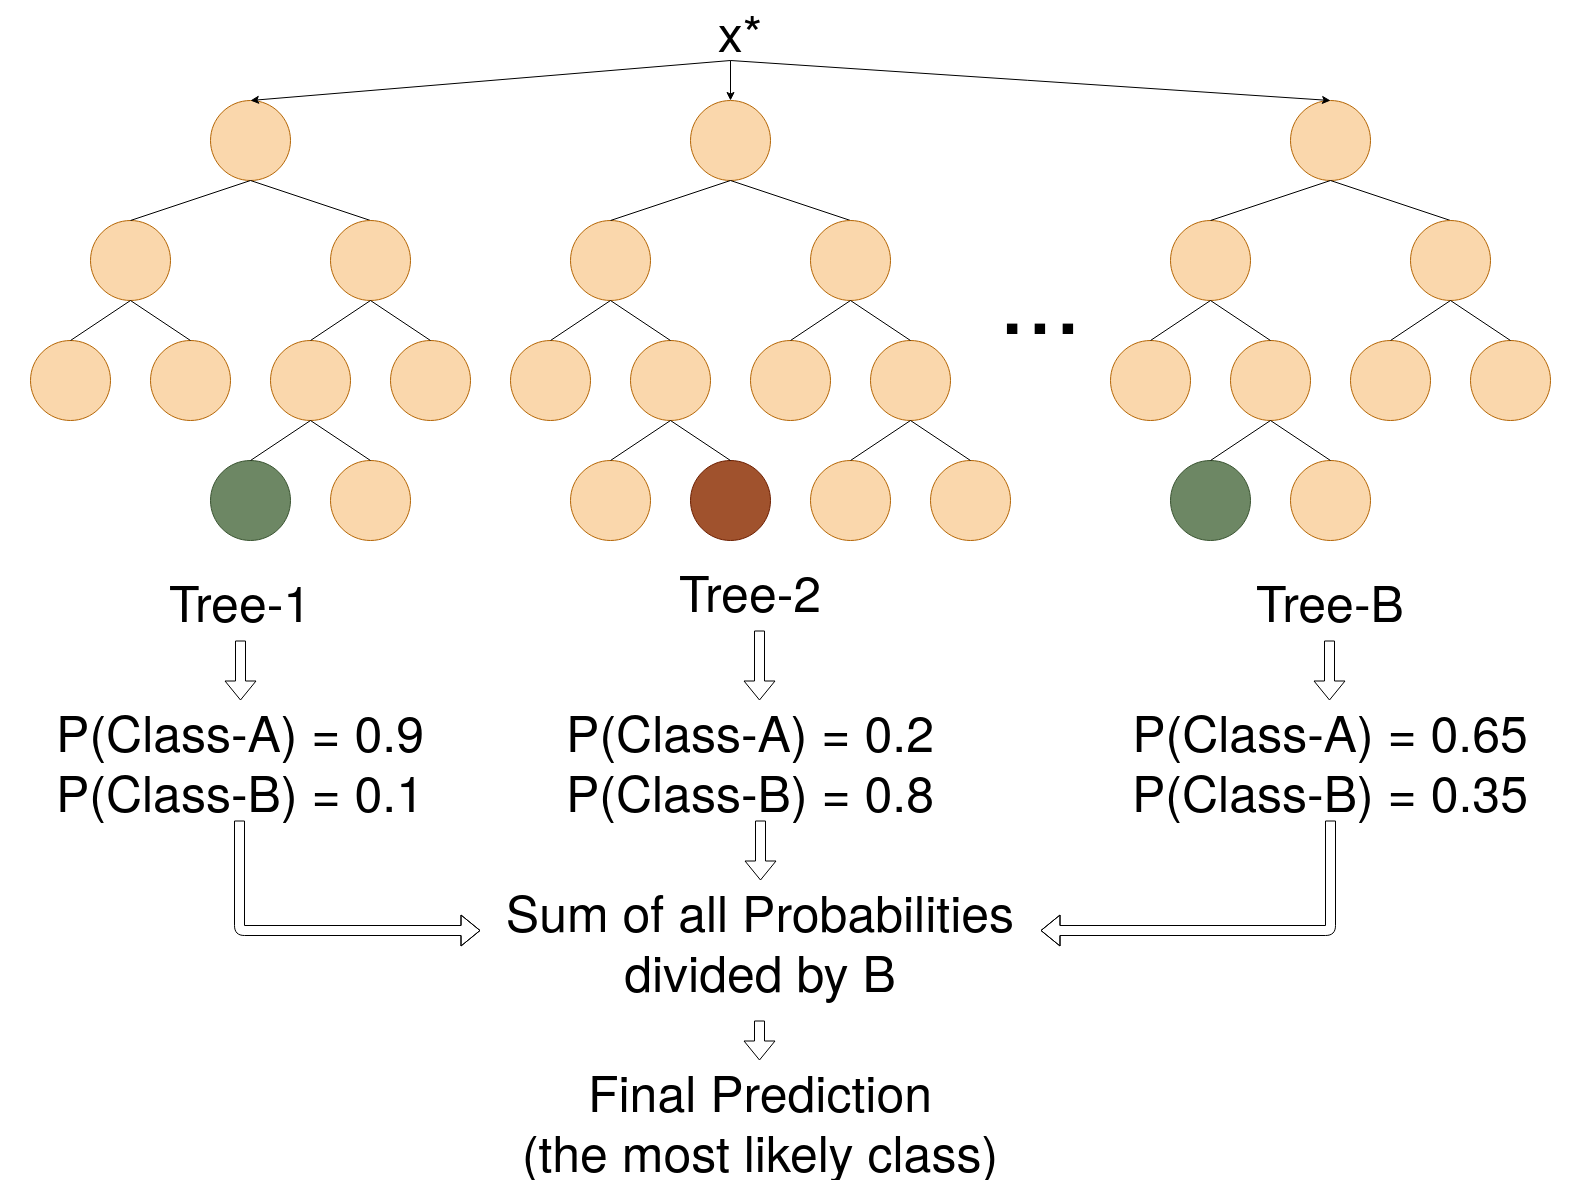
\includegraphics[height=0.7\textheight]{images/soft.png}
    \end{figure}
\end{frame}
\begin{frame}
    \frametitle{Mathematical Concept}
    \framesubtitle{The Expected Generalization Error of $\boldsymbol{T_{D,\theta}}$}
        \onslide<1->{\quad Given $D = X \cup Y$,\\
        \quad the expected generalization error of $T_{D,\theta}$ is
            \begin{align*}\label{eq:exp_gen_error}
                \boldsymbol{Err}(T_{D,\theta}(X)) = \mathbb{E}_{X,Y}\{L(Y, T_{D,\theta}(X)) \}
            \end{align*}
        \quad where $L(Y, T_{D,\theta}(X))$ is the loss function.\\
        }
        \bigbreak
        \onslide<2->{
            The decomposition of $\boldsymbol{Err}(T_{D,\theta})$ is
            \begin{block}{}
                \begin{center}
                    $\boldsymbol{Err}(T_{D,\theta}(X)) = \boldsymbol{Err}(\phi_{\beta}(X)) + 
                    [Bias(T_{D,\theta}(X))]^2 + Var(T_{D,\theta}(X))$
                \end{center}
            \end{block}
        }
        \onslide<3->{
        \quad similarly
        \begin{block}{}
            \begin{center}
                    $\boldsymbol{Err}(\boldsymbol{RF}_{D, \Theta}(X))
                    = \boldsymbol{Err}(\phi_{\beta}(X))
                    + [Bias(\boldsymbol{RF}_{D, \Theta}(X))]^2 
                    + Var(\boldsymbol{RF}_{D, \Theta}(X))$
                \end{center}
        \end{block}
        \quad where $\Theta = \{\theta_{1},\theta_{2},\,...\,, \theta_{B}\}$.
        }
    %\onslide<3->{where}
    %\begin{align*}
    %    \onslide<4->& \boldsymbol{Err}(\phi_{\beta}) =  \text{Bayes Error}\\
    %    \onslide<5->& [Bias(T_{D,\theta})]^2 = (\phi_{\beta}(x) 
    %                                            -\mathbb{E}_{D}\{T_{D,\theta}(x)\})^2 \\
    %    \onslide<6->& Var(T_{D,\theta}) = \mathbb{E}_{D}\{(\mathbb{E}_{D}(T_{D,\theta}(x)) 
    %                                        - T_{D,\theta}(x))^2\} = \sigma_{D,\theta}^2(x)
    %\end{align*}
\end{frame}

\begin{frame}[t]
    \frametitle{Mathematical Concept}
    \framesubtitle{Residual Error}
    \onslide<1->{    
        \begin{block}{}
        \begin{center}
            $\boldsymbol{Err}(\boldsymbol{RF}_{D, \Theta}(X))
                = \boldsymbol{Err}(\phi_{\beta}(X))
                \semitransp{+ [Bias(\boldsymbol{RF}_{D, \Theta}(X))]^2 
                + Var(\boldsymbol{RF}_{D, \Theta}(X))}$
        \end{center}
        \end{block}
    }
    \bigbreak
    \onslide<2->{
        \quad Theoretically, given the probability distribution of P(X,Y)\\
        \quad Bayes Model $\phi_{\beta}$ i.e the best possible model can be derived\\
        \quad and $\boldsymbol{Err}(\phi_{\beta})$ can be calculated \cite{louppe2014understanding}.\\
    }
    \bigbreak
    \onslide<3->{
        \quad For comparison of $\boldsymbol{Err}(T_{D,\theta}(X))$ and $\boldsymbol{Err}(\boldsymbol{RF}_{D, \Theta}(X))$\\
        \quad the residual error is the same.\\
    }
    \bigbreak
    \onslide<4->\quad \textbf{Result:} Ensembling has no effect on Bayes Error.

    %\onslide<2->{
    %    Theoretically, there exists a model that minimizes 
    %    the generalization error and can be derived analitically 
    %    independent of the model \cite{louppe2014understanding}.\\
    %    Conditioning the expected generalization error on X gives:
    %    \begin{center}
    %        $\mathbb{E}_{X,Y} \{L(Y, \phi_{\beta}(X))\} = \mathbb{E}_{X}\{\mathbb{E}_{Y|X}\{L(Y, \phi_{\beta}(X)) \} \}$
    %    \end{center}
    %}
    %\onslide<3->{
    %    Point-wise minimization of inner term yields:
    %    \begin{center}
    %        $\phi_{\beta} = \underset{c \in Y}{argmin} \; \mathbb{E}_{Y|X=x}\{L(Y,c)\}$
    %    \end{center}
    %}
    %\vspace{-2mm}
    %\onslide<4->\quad Bayes Model $\phi_{\beta}$ is best attainable model.\\
    %\smallbreak
    %\onslide<5->\quad $\boldsymbol{Err}(\phi_{\beta}(X))$ is the irreducible error.\\
    %\smallbreak
    %\onslide<6->\quad \textbf{Result:} Ensembling has no effect on Bayes Error.
\end{frame}

\begin{frame}[t]
    \frametitle{Mathematical Concept}
    \framesubtitle{Bias}
    \onslide<1->{    
        \begin{block}{}
            \begin{center}
                $\boldsymbol{Err}(\boldsymbol{RF}_{D, \Theta}(X))=
                \semitransp{\boldsymbol{Err}(\phi_{\beta}(X)) +}
                \nontransp{[Bias(\boldsymbol{RF}_{D, \Theta}(X))]^2 }
                \semitransp{+ Var(\boldsymbol{RF}_{D, \Theta}(X))}$
            \end{center}
        \end{block}
    \center{With Squared Loss Function: 
            $L(Y,T_{D,\theta}(X))=\mathbb{E}_{D}\{(Y-T_{D,\theta}(X))^2\}$
            }
    }
    \onslide<2->{
        \begin{block}{$Bias^2$ of Tree}
            \begin{center}
                $[Bias(T_{D,\theta}(X))]^2 = (\phi_{\beta}(X) -\mathbb{E}_{D}\{T_{D,\theta}(X)\})^2$
            \end{center}
        \end{block}
    }
    \onslide<3->{
        \begin{block}{$Bias^2$ of Random Forest}
            \begin{center}
                $[Bias(\boldsymbol{RF}_{D, \Theta}(X))]^2 
                = (\phi_{\beta}(X) - \mathbb{E}_{D,\Theta}\{\boldsymbol{RF}_{D, \Theta}(X))\})^2$ 
            \end{center}
        \end{block}
    }
    \onslide<4->\center{
    We need $\mathbb{E}_{D,\theta}\{T_{D, \theta}(X))\}$ and 
    $\mathbb{E}_{D,\Theta}\{\boldsymbol{RF}_{D, \Theta}(X))\}$ for comparison.}

\end{frame}

\begin{frame}[c]
    \frametitle{Mathematical Concept}
    \framesubtitle{Bias: The Expected Value}
    \onslide<1->{
        We can define $\mathbb{E}_{D}\{T_{D,\theta}(X)\} = \mu_{D,\theta}(X)$\\
    }
    \bigbreak
    \onslide<1->{
        Random Forest Estimator for regression is;
        \vspace{-3mm}
        \begin{align*}
            \boldsymbol{RF}_{D, \Theta}(X) = \dfrac{1}{B}\sum_{b = 1}^{B}T_{D,\theta_{b}}(X)
        \end{align*}
    }
    \onslide<2->{Taking expectation gives;}
        \vspace{-5mm}
        \begin{align*}
            \onslide<2->\mathbb{E}_{D, \Theta}\{\boldsymbol{RF}_{D, \Theta}(X) \} 
            & = \mathbb{E}_{D, \Theta}\{\dfrac{1}{B}\sum_{b = 1}^{B}T_{D,\theta_{b}}(X)\}  \\
            \onslide<3->& = \dfrac{1}{B}\sum_{b=1}^{B}\mathbb{E}_{D,\theta_{b}}\{T_{D, \theta_{b}}(X)\} 
            & \text{($\theta$'s are i.i.d.)}\\
            \onslide<4->& = \mu_{D,\theta}(X)
        \end{align*}
\end{frame}

\begin{frame}[t]
    \frametitle{Mathematical Concept}
    \framesubtitle{Bias Comparison}
    \begin{block}{}
        \begin{center}
            $\boldsymbol{Err}(\boldsymbol{RF}_{D, \Theta}(X)) =
            \semitransp{\boldsymbol{Err}(\phi_{\beta}(X)) +}
            \nontransp{[Bias(\boldsymbol{RF}_{D, \Theta}(X))]^2 }
            \semitransp{+ Var(\boldsymbol{RF}_{D, \Theta}(X))}$
        \end{center}
    \end{block}
    \vspace{0.5cm}
    \begin{block}{$Bias^2$ of Tree}        
        \begin{center}
            $[Bias(T_{D,\theta})(X)]^2 = (\phi_{\beta}(X) - \mu_{D,\theta}(X)\})^2$
        \end{center}
    \end{block}
    \bigbreak
    \begin{block}{$Bias^2$ of a Random Forest}
        \begin{center}
            $[Bias(\boldsymbol{RF}_{D,\Theta})(X)]^2 = (\phi_{\beta}(X) - \mu_{D,\theta}(X))^2$
        \end{center}
    \end{block}
    \bigbreak
    \onslide<2->{\textbf{Result:} Ensembling trees has no effect on bias.}
\end{frame}
\begin{frame}[t]
    \frametitle{Mathematical Concept}
    \framesubtitle{Variance: Correlation Coefficient}
    \onslide<1->{    
        \begin{block}{}
            \begin{center}
                $\boldsymbol{Err}(\boldsymbol{RF}_{D, \Theta}(X)) =
                \semitransp{\boldsymbol{Err}(\phi_{\beta}(X)) +}
                \semitransp{[Bias(\boldsymbol{RF}_{D, \Theta}(X))]^2+}
                \nontransp{Var(\boldsymbol{RF}_{D, \Theta}(X))}$
            \end{center}
        \end{block}
    }
    \onslide<2->{
        $\forall T_{D,\theta'}$,$T_{D,\theta''}$ such that  $\theta' \neq \theta''$,\\
        we can define the correlation coefficient as follows
        \begin{center}
            $\rho(X)
            = \dfrac{\mathbb{E}_{D,\theta',\theta''}\{T_{D,\theta'}(X) T_{D,\theta''}(X)\} 
            - \mu_{D,\theta}^2(X)}{\sigma_{D,\theta}^2(X)}$
        \end{center}
        \quad where $\sigma_{D,\theta}^2(X) = \mathbb{V}_{D,\theta}\{T_{D,\theta}(X)\}$.
    }
    \bigbreak
    \onslide<3->{
        \begin{itemize}
        \item Highly correlated trees $\implies$ $\rho(X)$ is close to 1\\
        \bigbreak
        \item Non-correlated trees $\implies$ $\rho(X)$ is close to 0
    \end{itemize}
    }
\end{frame}
\begin{frame}[t]
    \frametitle{Mathematical Concept}
    \framesubtitle{Variance Comparison}
    \onslide<1->{    
        \begin{block}{}
            \begin{center}
                $\boldsymbol{Err}(\boldsymbol{RF}_{D, \Theta}(X)) =
                \semitransp{\boldsymbol{Err}(\phi_{\beta}(X)) +}
                \semitransp{[Bias(\boldsymbol{RF}_{D, \Theta}(X))]^2+}
                \nontransp{Var(\boldsymbol{RF}_{D, \Theta}(X))}$
            \end{center}
        \end{block}
        \begin{block}{Variance of Random Forest}
            \begin{center}
                $\mathbb{V}_{D, \Theta}\{
                \boldsymbol{RF}_{D, \Theta}(X) \} 
                = \rho(X)\sigma^2_{D,\theta}(X) + \dfrac{1-\rho(X)}{B}\sigma^2_{D,\theta}(X)$
            \end{center}
        \end{block}
    }
    \bigbreak
    \onslide<2->{
        \quad As $B \rightarrow \infty$, $\mathbb{V}_{D,\Theta}\{\boldsymbol{RF}_{D, \Theta}(X) \}$ 
        converges to $\rho(X)\sigma^2_{D,\theta}(X)$.
    }
    \bigbreak
    \onslide<3->{
        \quad Due to randomization $\rho(X) < 1$
        \begin{block}{}
            \center{
                $\implies \mathbb{V}_{D,\Theta}\{\boldsymbol{RF}_{D, \Theta}(X) \}
                = \rho(x)\sigma^2_{D,\theta}(X)
                < \sigma^2_{D,\theta}(X) = \mathbb{V}_{D,\theta} \{T_{D,\theta}(X)\} $.
            }
        \end{block}
    }
    \bigbreak
    \onslide<4->{
        \quad \textbf{Result:}Ensembling trees decreases the variance.
    }
\end{frame}
%\begin{frame}
%    \frametitle{Loss Functions}
%\begin{block}{Regression}
%            Squared Loss Function
%            \begin{align*}
%                L(Y, T_{D, \theta}(x)) = (Y - T_{D, \theta}(x))^2\\
%                \boldsymbol{Err}(T_{D,\theta}) = \mathbb{E}_{X,Y}\{ (Y - T_{D, \theta}(x))^2 \}
%            \end{align*}
%        \end{block}
%\begin{block}{Classification}    
%            Zero-One Loss Function
%            \begin{align*}
%                L(Y, T_{D,\theta}(X)) = 1 (Y \neq T_{D, \theta}(X))
%            \end{align*}                
%            \begin{align*}
%                \boldsymbol{Err'}(T_{D,\theta}) & = \mathbb{E}_{X,Y}\{ 1(Y \neq T_{D, \theta}(X)) \}\notag \\
%                & = P(Y \neq T_{D, \theta}(X))
%            \end{align*}
%        \end{block}
%\end{frame}
%\begin{frame}
%    \frametitle{Bayes Model cont.}
%    \begin{block}{Regression}
%        \begin{align*}
%            \phi_{\beta} & = \underset{c \,\in\, Y}{argmin} \; \mathbb{E}_{Y|X=x}\{(Y-c)^2 \} \notag\\
%            \phi_{\beta} & = \mathbb{E}_{Y|X=x}\{Y\}\\
%            \boldsymbol{Err}(\phi_{\beta}) & = \mathbb{E}_{Y|X=x}\{(Y-\phi_{\beta}(x))^2 \}
%        \end{align*}
%    \end{block}
%    \begin{block}{Classification}
%        \begin{align*}
%            \phi_{\beta}' & = \underset{c \,\in\, Y}{argmin} \; \mathbb{E}_{Y|X=x}\{L(Y,c) \} \notag\\
%            \phi_{\beta}' & = \underset{c \,\in\, Y}{argmax} \; P(Y = c \,| X = x)\\
%            \boldsymbol{Err}(\phi_{\beta}') & = P(Y \neq \phi_{\beta}'(x) )
%        \end{align*}
%    \end{block}
%\end{frame}